\subsection{Implementierung AppSync und DynamoDB}
Der erste benötigte Dienst für die Webanwendung ist die GraphQL API.
Mit \verb+amplify add api+ startet der Konfigurationsassistent:

\begin{verbatim}
Please select from one of the below mentioned services: GraphQL
Provide API name: amplify-kumo-api
Choose the default authorization type for the API API key
Enter a description for the API key: My-Dev-ApiKey
After how many days from now the API key should expire (1-365): 7
Do you want to configure advanced settings for the GraphQL API: No
Do you have an annotated GraphQL schema? No
Do you want a guided schema creation? Yes
What best describes your project:
Single object with fields (e.g., “Todo” with ID, name, description)
Do you want to edit the schema now? Yes

\end{verbatim}

Da die Authentifizierung mit Cognito erst zu einem späteren Zeitpunkt hinzugefügt wird, erfolgt sie solange mittels API Key.
Nach dem bestätigen des letzten Schrittes, öffnet sich das GraphQL Schema, \verb+schema.graphql+ welches im Projektverzeichnis erstellt wurde. (siehe \ref{GraphQL} \nameref{GraphQL} für weitere Informationen.)
In dieser Datei werden alle benötigten Objekttypen erstellt.
Für den ersten Schritt wird nur ein Objekt mit dem Namen Account generiert:

\begin{verbatim}
type Account @model {
  id: ID!
  accountid: String!
  name: String!
  email: String!
  num: Int!
  status: String!

}

\end{verbatim}

Alle angegeben Felder müssen im späteren Verlauf von der Lambda-Funktion abgerufen und gespeichert werden.
Mit dem Befehl \verb+amplify push+ wird die API in der Cloud bereitgestellt.
Im folgenden Dialog besteht die Möglichkeit alle möglichen Mutationen und Queries generieren zu lassen.
\begin{verbatim}
# You will be walked through the following questions for GraphQL code generation
Do you want to generate code for your newly created GraphQL API? Y
Choose the code generation language target: javascript
Do you want to generate/update all possible GraphQL operations - queries, mutations and subscriptions? Y
\end{verbatim}

Sobald der Prozess fertig gestellt ist, sind die Dienste AWS AppSync und DynamoDB konfiguriert.
In der Webkonsole kann überprüft werden, ob der Vorgang erfolgreich war.

\begin{figure}[htbp]
    \centering
    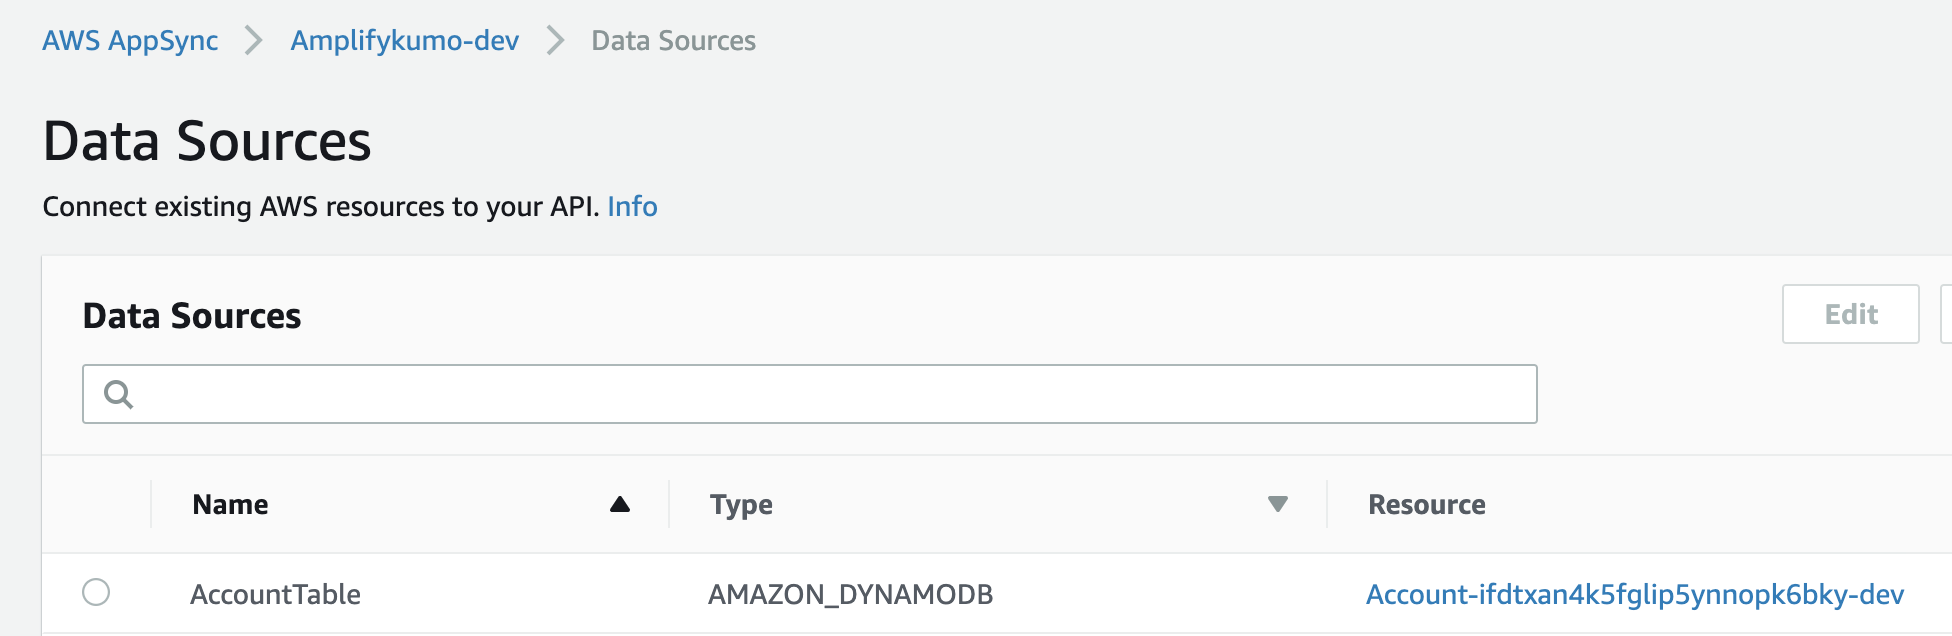
\includegraphics[width=1.0\textwidth]{50-Implementierung/AppSync-DynamoDB.png}
    \caption{Ansicht AWS AppSync in der Webkonsole}
    \label{fig:meine-grafik}
\end{figure}

In der Ansicht von AppSync sieht man, dass eine DynamoDB-Tabelle passend zum GraphQL Objekttyp erstellt wurde.
In dem React Frontend kann jetzt mit dem AppSync SDK auf diese Datenbank zugegriffen werden.
Bevor das Frontend jedoch Anfragen an die Datenbank ausführen kann, muss Lambda konfiguriert werden, sodass Daten gespeichert werden.

\subsection{Implementierung Lambda}
Die gesamte Backend-Logik wird durch Lambda realisiert.
Wie bereits erwähnt soll Lambda in regelmäßigen Abständen ausgeführt werden, um die Daten aktuell zu halten.
Mit dem Befehl \verb+amplify add function+ startet Amplify den Prozess:

\begin{verbatim}
[143302S0:amplify-kumo] master # amplify add function
Using service: Lambda, provided by: awscloudformation
  Provide a friendly name for your resource to be used as a label for this category in the project: getallaccounts
  Provide the AWS Lambda function name: getallaccounts
  Choose the function runtime that you want to use: NodeJS
  Choose the function template that you want to use: Hello World
  Do you want to access other resources created in this project from your Lambda function? Yes
  Select the category: storage
  Do you want to invoke this function on a recurring schedule? Yes
  At which interval should the function be invoked: Daily
  Select the start time (use arrow keys): 06:35 PM
Successfully added resource getallaccounts locally.
\end{verbatim}

Bevor spezielle Auslöser für die Funktion erstellt werden, reicht eine tägliche Ausführung aus.
In der Regel werden neue AWS Accounts in Abständen von 2-3 Wochen erstellt.
Daher hat ein zeitnaher Auslöser zu Beginn keine hohe Priorität.
Nachdem Amplify die Lambda-Funktion erstellt hat, kann diese direkt bearbeitet werden.

Der vollständige Code befindet sich im Anhang. (Siehe XXXX)
Die Lambda-Funktion besteht aus den Funktionen \verb+getCallerIdentity()+,
\verb+getCrossAccountCredentials()+, \verb+listAllAccounts()+ sowie \verb+writeAllDynamoDBItems()+.
Eine Schwierigkeit war es, eine Identität im \verb+Cbc-Master+ anzunehmen.
Die Lambda-Funktion befindet sich im AWS Account \verb+Cbc-Clouds-Sandbox+ und muss auf den Account \verb+Cbc-Master+ zugreifen.

\subsubsection{Accountübergreifender Zugriff}

Im Account \verb+Cbc-Master+ wird eine IAM-Rolle benötigt, die der Lambda-Funktion aus dem anderen Account Zugriff gewährt.
Mit IAM-Rollen können anderen Benutzeraccounts oder AWS-Dienste Zugriff temporäre Anmeldeinformationen erhalten, die Accountübergreifend funktionieren.
Die IAM-Rolle erhält die Berechtigung \verb+AWSOrganizationsReadOnlyAccess+ und hat eine Vertrauensstellung zu der Lambda-Funktion.
Das folgende Bild zeigt die konfigurierte Vertrauensstellung zwischen Lambda-Funktion im \verb+Cbc-Clouds-Sandbox+ und IAM-Rolle im \verb+Cbc-Master+ Account.


\begin{figure}[htbp]
    \centering
    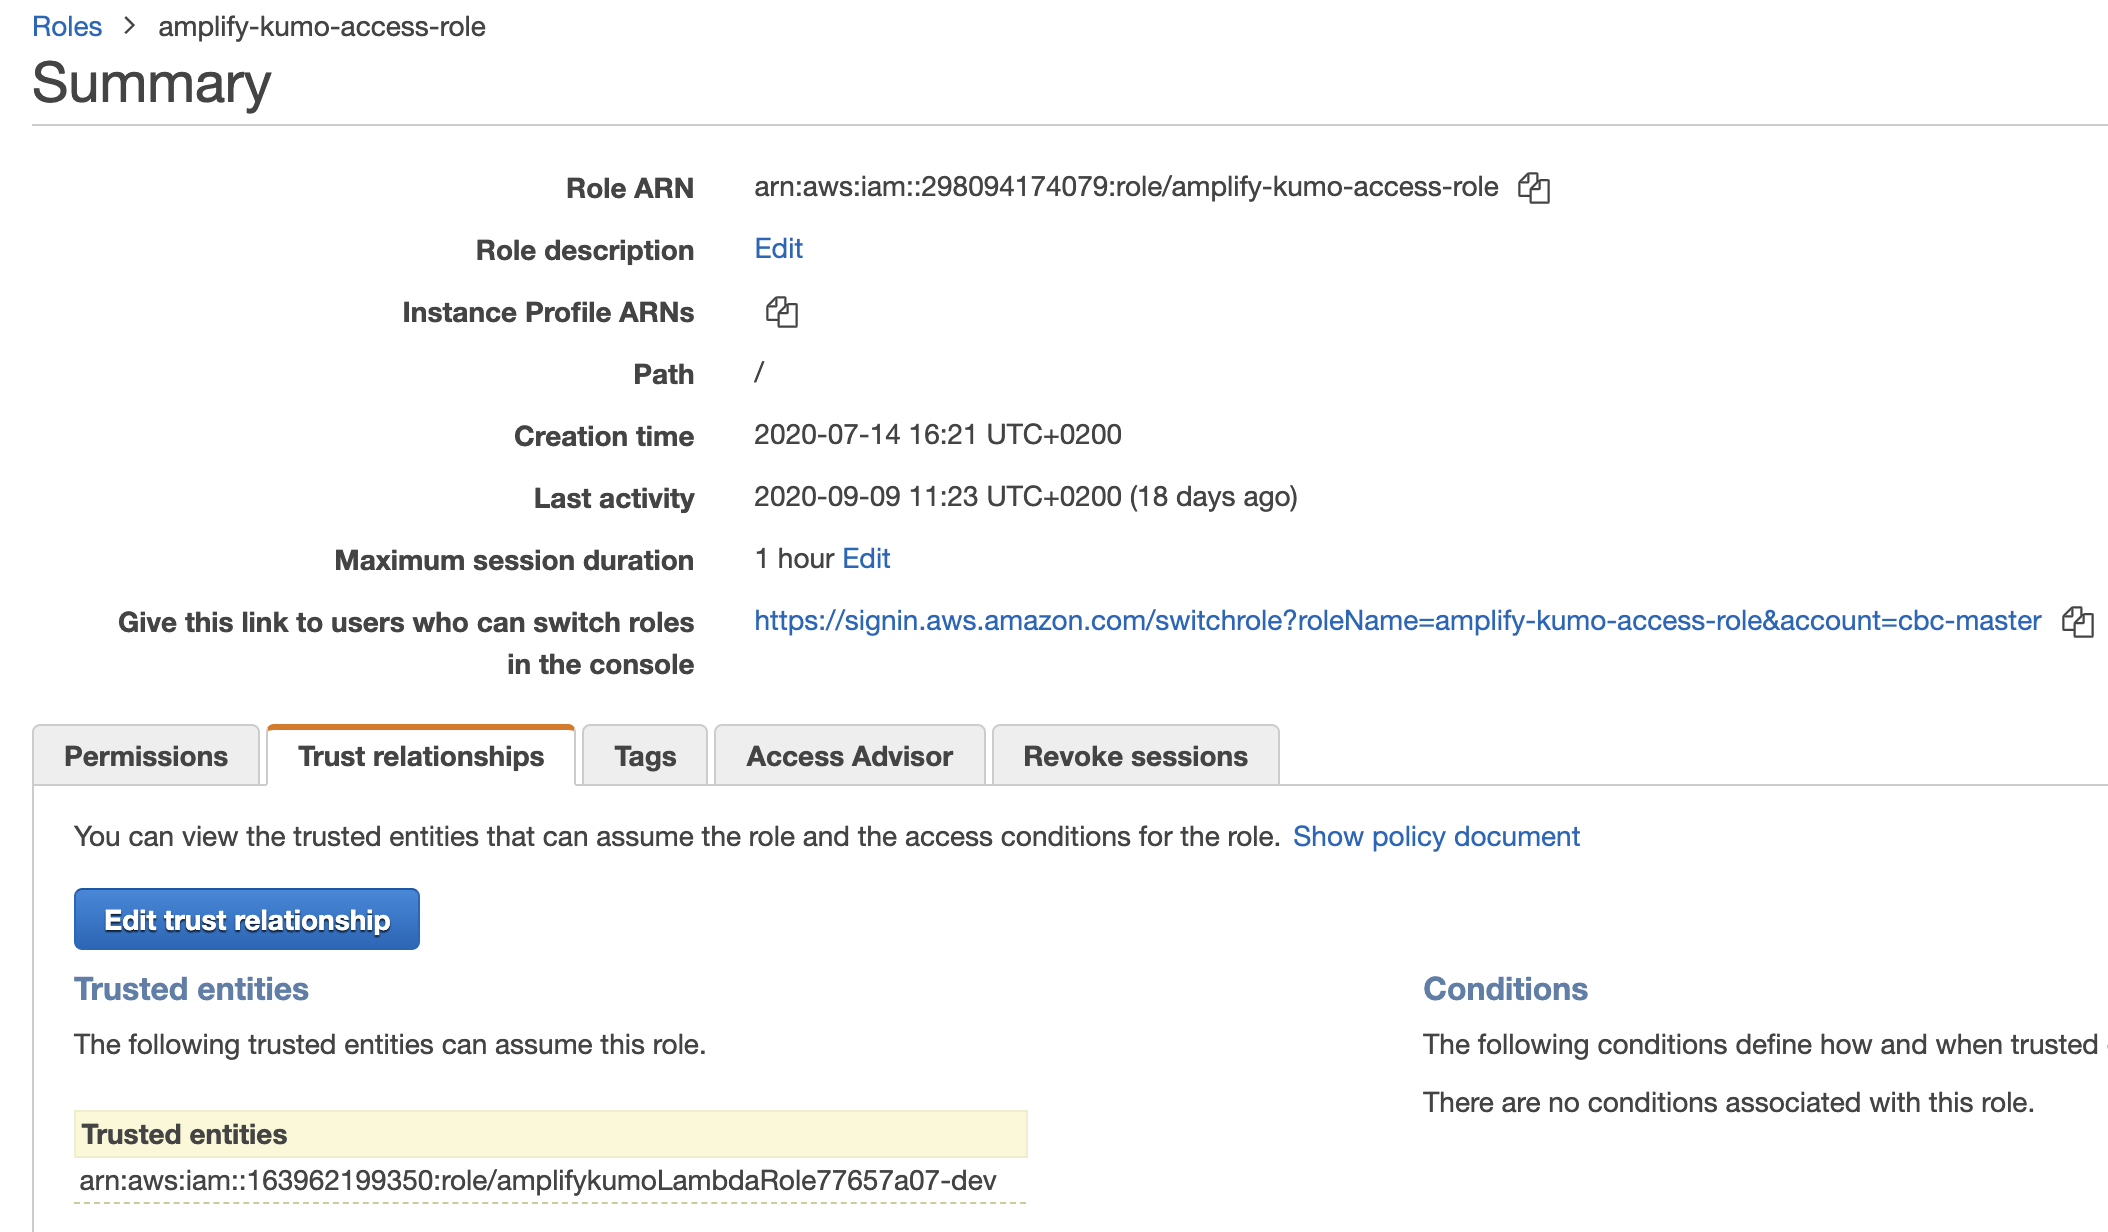
\includegraphics[width=1.0\textwidth]{50-Implementierung/IAM-Rolle.png}
    \caption{Vertrauensstellung zwischen beiden Accounts}
    \label{fig:meine-grafik}
\end{figure}


Dieser Zugriff auf den Account muss in Lambda programmiert werden.
Dazu dienen die Funktionen \verb+getCallerIdentity()+ und \verb+getCrossAccountCredentials()+.
\verb+getCallerIdentity()+ ist eine Hilfsfunktion und gibt die aktuelle Identität zurück.
So ist es leichter zu überprüfen ob die Rolle im \verb+Cbc-Master+ Account erfolgreich angenommen wurde.
Das eigentliche Übernehmen der IAM-Rolle erledigt \verb+getCrossAccountCredentials()+.
Es wird ein neues AWS Service-Objekt für den Dienst AWS Organizations erstellt und mithilfe der Funktion \verb+sts.assumeRole()+ ein temporärer Zugang im Master-Account erstellt.

Ein Service-Objekt wird benötigt, um auf Service-Funktionen über die JavaScript-API zugreifen zu können.
Die meisten AWS-Dienste bieten mindestens ein passendes Service-Objekt an.
In der Lambda-Funktion muss dementsprechend ein Service-Objekt für die Dienste AWS Organizations, DynamoDB und für die Hilfsfunktion AWS STS \footnote{STS steht für Security Token Service und ermöglicht die Bereitstellung von temporären Anmeldeinformationen.} erstellt werden.
\cite[]{ServiceObject}

Für DynamoDB reicht etwa folgender Befehl aus um eine passendes Service-Objekt zu erstellen:
\begin{verbatim}
    var docClient = new AWS.DynamoDB.DocumentClient
\end{verbatim}

Die Lambda-Funktion und die DynamoDB-Tabelle befinden sich im selben Account.
Auch besitzt die Lambda-Funktion bereits alle nötigen Berechtigungen, da diese durch Amplify gesetzt wurden.

Für AWS Organizations müssen bei der Erstellung des Service-Objekts zusätzlich die temporären Anmeldeinformation mitgegeben werden, da sich der Dienst in einem anderen Account befindet.
Außerdem muss die Region geändert werden. AWS Organizations ist ein Dienst, der nur in der Region \verb+us-east-1+ betrieben wird.
Für den Vorgang wird die Funktion \verb+getCrossAccountCredentials()+ benötigt:

\begin{verbatim}
    var accessparams = await getCrossAccountCredentials();

    const cbc_master_orgs = new AWS.Organizations({
        credentials: accessparams,
        region: 'us-east-1'
      });
\end{verbatim}

Im ersten Schritt werden temporäre Anmeldeinformation abgerufen und anschließend dem Service-Objekt übergeben.
Dadurch ist es der Funktion möglich die Funktion \verb+listAllAccounts()+ mit einer anderen Identität auszuführen.

\subsubsection{Asynchrone Verarbeitung mit NodeJS}

Alle vier Funktionen werden im Handler der Funktion nacheinander ausgeführt.
Neben den unterschiedlichen IAM-Rollen war die Sicherstellung der asynchronen Abarbeitung ein wichtiger Aspekt bei der Programmierung.
Alle Funktionen durften nicht gleichzeitig ausgeführt werden, da sie voneinander abhängig waren.
Damit die Funktion \verb+listAllAccounts()+ erfolgreich war, musste zuvor Identität des Master-Accounts angenommen werden.
Zudem muss die Funktion \verb+writeAllDynamoDBItems()+ auf die Fertigstellung von \verb+listAllAccounts()+ warten, da sie sonst keine Daten zum speichern hat.

NodeJS arbeitet Single-Threaded.
Das bedeutet, dass zu einem Zeitpunkt immer nur genau eine Aufgabe erledigt werden kann.
Aufgrund der Abhängigkeit der Funktionen muss eine asynchrone Abarbeitung stattfinden.
Zur Option stehen dazu Callbacks, Promises oder eine Implementierung mit async/await.
Ein Callback ist eine Funktion die an eine weitere Funktion weitergegeben wird.
So wird sichergestellt, dass die zweite Funktion erst aufgerufen wird, sobald die Erste beendet ist.
Das Problem von Callbacks ist die große Unübersichtlichkeit bei mehreren Funktionen
Das immer tiefere verschachteln von Funktionsaufrufen wird auch als \glqq Callback-Hölle\grqq{} bezeichnet.
Promises ermöglichen die selbe Funktionalität wie Callbacks, nur ohne die Verschachtelung.
\glqq Ein Promise ist ein Objekt, das die finale Beendigung einer asynchronen Operation repräsentiert.
Je nachdem, ob die Operation erfolgreich oder fehlerhaft beendet wurde, wird das Promise entsprechend gekennzeichnet. \grqq{} \cite[]{Promises}
Mit der Option \verb+.then()+ kann sichergestellt werden, dass die Operation beendet sein muss bevor der nächste Codeblock beginnt.
Die letzte Möglichkeit ist die Verwendung von \verb+async/await+, welche auf Promises basiert jedoch eine verständlichere Syntax ermöglicht.
Eine Funktion kann mit \verb+async+ als Asynchron deklariert werden.
Innerhalb einer asynchronen Funktion kann mit dem Operator \verb+await+ auf die Erfüllung des Promises gewartet werden.
Es ist auch möglich den Operator \verb+await+ in einer Funktion mehrmals zu verwenden.

Die Lambda-Funktion nutzt Promises und \verb+async/await+ zu einem großen Teil aus um die Funktionalität gewährleisten zu können.
Der Event Handler wird als Asnychron deklariert und innerhalb des Handlers werden alle oben genannten Funktion nacheinander aufgerufen.
Die genaue Verwendung der asnychronen Abläufe befindet sich im Anhang.


\subsection{Implementierung Cognito}

Im Abschnitt \ref{CognitoEntscheidung} \nameref{CognitoEntscheidung} wurde bereits erwähnt, dass Amplify in Kombination mit Cognito
alle benötigten Module für ine vollständige Authentifizierung beinhaltet.
Um eine Authentifizierung für Amplify hinzuzufügen muss der Befehl \verb+amplify add auth+ ausgeführt werden.

\begin{verbatim}
  Do you want to use the default authentication and security configuration? Default configuration
  How do you want users to be able to sign in? E-Mail
  Do you want to configure advanced settings?  No, I am done.
\end{verbatim}

Nach dem Befehl \verb+amplify push+ wird ein Cognito User Pool inklusive App Clients erstellt.
Über die Webkonsole besteht im Anschluss Option die Option MFA zu aktivieren.

\subsubsection{Probleme mit AzureAD}

Probleme mit Authentifizierung
https://medium.com/@zippicoder/setup-aws-cognito-user-pool-with-an-azure-ad-identity-provider-to-perform-single-sign-on-sso-7ff5aa36fc2a

Customize Auth
https://blog.kylegalbraith.com/2020/03/31/customizing-the-aws-amplify-authentication-ui-with-your-own-react-components/

Blöde Lösung: https://dunlop.geek.nz/aws-cognito-azure-ad-react-amplify/

\subsection{Implementierung Hosting und Veröffentlichung}
